\documentclass[11pt]{article}
\usepackage{natbib}
\usepackage{amsmath}
\usepackage{lscape}
\usepackage{listings}
\usepackage{color}
\usepackage{url}


\usepackage{geometry}
\usepackage{pdflscape}

\definecolor{dkgreen}{rgb}{0,0.6,0}
\definecolor{gray}{rgb}{0.5,0.5,0.5}
\definecolor{mauve}{rgb}{0.58,0,0.82}

\lstset{frame=tb,
  language=C,
  aboveskip=3mm,
  belowskip=3mm,
  showstringspaces=false,
  columns=flexible,
  basicstyle={\small\ttfamily},
  numbers=none,
  numberstyle=\tiny\color{gray},
  keywordstyle=\color{blue},
  commentstyle=\color{dkgreen},
  stringstyle=\color{mauve},
  breaklines=true,
  breakatwhitespace=true
  tabsize=3
}

%Gummi|065|=)
\title{\textbf{Project Report}}
\author{Lucas Sa \\
George Washington University \\
{\tt lucastsa@gwu.edu}}
\date{April, 2014}
\usepackage{graphicx}
\begin{document}

\maketitle

\section{Introduction}

\subsection{Objective}
The objective of this project was to implement a linear cryptanalysis attack against the Substitution-Permutation Network (SPN) created in Homework 2 in order to recover at least eight bits of the key. The original cipher consisted of six rounds, but the SPN used for this project has only four rounds, as the section below explains.

\subsection{The Cipher}

The cipher consists of a simple 4-round SPN as explained in \emph{Cryptography: Theory and Practice}\cite{stinson2005cryptography}, whose the Substitution-Box (S-box) and the Permutation are shown in Table \ref{tab:sbox} and Table \ref{tab:pbox} respectively.\footnote{In this report, all bit indexes starts on 0 and refer to the least significant bit of the binary string.}


\begin{table}
	\small
	\setlength{\tabcolsep}{5pt}
    \centering
    \begin{tabular}{|l|l|l|l|l|l|l|l|l|l|l|l|l|l|l|l|l|}
    \hline
	\textbf{input} & 0 & 1 & 2 & 3 & 4 & 5 & 6 & 7 & 8 & 9 & 10 & 11 & 12 & 13 & 14 & 15  \\ \hline
	\textbf{output} & 60 & 12 & 9 & 11 & 39 & 52 & 1 & 36 & 41 & 50 & 53 & 26 & 28 & 33 & 8 & 42 \\ \hline \hline

	\textbf{input} & 16 & 17 & 18 & 19 & 20 & 21 & 22 & 23 & 24 & 25 & 26 & 27 & 28 & 29 & 30 & 31  \\ \hline 
	\textbf{input} & 19 & 45 & 35 & 46 & 62 & 59 & 4 & 13 & 6 & 14 & 40 & 49 & 58 & 38 & 47 & 63 \\ \hline \hline

	\textbf{input} & 32 & 33 & 34 & 35 & 36 & 37 & 38 & 39 & 40 & 41 & 42 & 43 & 44 & 45 & 46 & 47 \\ \hline
	\textbf{output} & 24 & 22 & 43 & 55 & 18 & 48 & 2 & 23 & 25 & 31 & 16 & 10 & 5 & 27 & 15 & 61 \\ \hline \hline
	
	\textbf{input} & 48 & 49 & 50 & 51 & 52 & 53 & 54 & 55 & 56 & 57 & 58 & 59 & 60 & 61 & 62 & 63 \\ \hline
	\textbf{output} & 44 & 3 & 29 & 7 & 21 & 20 & 54 & 57 & 32 & 17 & 30 & 56 & 34 & 51 & 37 & 0 \\ \hline 
	
    \end{tabular}
    \caption{S-box}
    \label{tab:sbox}
\end{table}


\begin{table}
\setlength{\tabcolsep}{3pt}
    \centering
    \begin{tabular}{|l|l|l|l|l|l|l|l|l|l|l|l|l|l|l|l|l|l|l|l|l|l|l|l|l|}
    \hline
$i$ & 0 & 1 &  2 &  3 & 4 & 5 &  6 &  7 & 8 & 9 & 10 & 11 & 12 & 13 & 14 & 15 & 16 & 17 & 18 & 19 & 20 & 21 & 22 & 23 \\ \hline
$\pi(i)$ & 0 & 6 & 12 & 18 & 1 & 7 & 13 & 19 & 2 & 8 & 14 & 20 &  3 &  9 & 15 & 21 &  4 & 10 & 16 & 22 &  5 & 11 & 17 & 23 \\ \hline
    \end{tabular}
    \caption{Permutation: bit index $i$ and new position $\pi(i)$}
    \label{tab:pbox}
\end{table}


\section{Methodology}

The approach to complete this project was almost entirely based on the Linear Cryptanalysis tutorial by Howard Heys. \cite{heys2002tutorial}

\subsection{Analyzing the S-Box and the Permutation}

The S-Box of the cipher has 6-bit input and output. In order to find good linear relations between the input and output bits, a Linear Approximation Table (see 64 x 64 Table \ref{tab:sbox_approx_table}) with input and output sums was constructed with the auxiliary code function \texttt{generate\_approx\_table}:

\begin{lstlisting}
void generate_approx_table() {
    char sbox_linear_approx[64][64];

    byte input, mask_input, mask_output;
    byte output, masked_input, masked_output;

    // initializing sbox_linear_approx
    memset(sbox_linear_approx, -32, 64*64);

    for (input=0; input < 64; input++) {
        output = SBOX[input];
        for (mask_input=0; mask_input < 64; mask_input++) {
            masked_input = input & mask_input;
            for (mask_output=0; mask_output < 64; mask_output++) {
                masked_output = output & mask_output;
                if (!get_parity(masked_input ^ masked_output))
                    sbox_linear_approx[mask_input][mask_output]++;
            }
        }
    }
}
\end{lstlisting}

Also with an auxiliary code, a number of expressions that hold with a bias $|\epsilon| > \frac{8}{64}$ were generated from the approximation table and manually analyzed. One interesting characteristic of this Permutation is that both the 0th and the 23th bits keep the same positions after the permutation, as shown in Table \ref{tab:pbox}.

In order to simplify the equations that derive a linear approximation for the entire network, the expression $X_5 = Y_5$  was chosen with a bias $\epsilon = \frac{-8}{64} = \frac{-1}{8}$. As the 23th bit of each round is the 5th ($X_5$) of the round's first box, such expression could be used to "pass through" all rounds up to the 23th bit of the ciphertext (see first two rounds of Figure \ref{fig:approx}).

Nevertheless, that would attack only one of the last round's S-boxes (six bits), and we should be able to recover at least eight bits. Therefore, for the third round, we use expression $X_5 = Y_1 \oplus Y_2 \oplus Y_4$, which has a slightly higher bias $\epsilon = \frac{10}{64}$ in order to reach S-boxes S41 and S43 (see Figure \ref{fig:approx}).

\begin{figure}[htp]
\centering
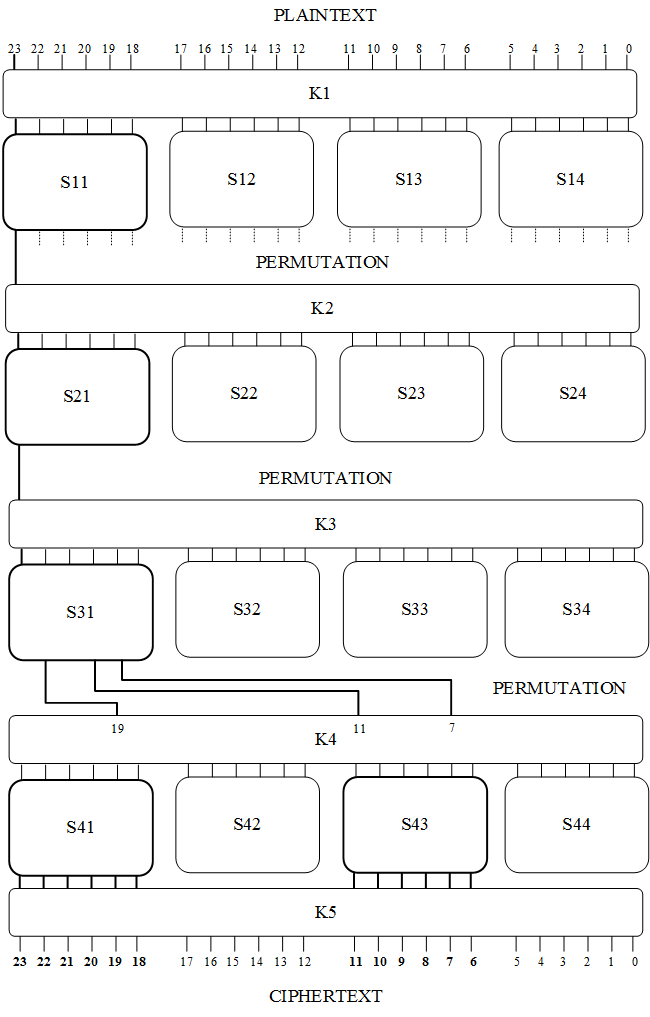
\includegraphics[scale=0.75]{SPN.png}
\caption{Linear Approximation. Several lines are omitted on purpose for simplicity. The actual "path" is bolder.}
\label{fig:approx}
\end{figure}


\subsection{Deriving a Linear Approximation}

In the previous section we showed:

\begin{equation}
 X_5 = Y_5 \\
\label{x5y5}
\end{equation}

\begin{equation}
 X_5 = Y_1 \oplus Y_2 \oplus Y_4\\
\label{x5y}
\end{equation}

Now, following the path shown in Figure \ref{fig:approx} and using the standard convention $U$ to represent S-box input string and $V$ the output string, we have $U_{1,23} = V_{1,23}$ in S-box S11 based on (\ref{x5y5}) with $\epsilon = \frac{-1}{8}$. As $U_{1,23} = P_{23} \oplus K_{1,23}$, we finally have:

\begin{equation}
V_{1,23} = P_{23} \oplus K_{1,23}
\label{r1}
\end{equation}

In round 2, we will continue with the S-box approximation (\ref{x5y5}) in $S21$, having $U_{2,23} = V_{2,23}$ with a bias $\epsilon = \frac{-1}{8}$. As $U_{2,23} = V_{1,23} \oplus K_{2,23}$, we have that:

\begin{equation}
V_{2,23} = V_{1,23} \oplus K_{2,23}
\label{r2}
\end{equation}


In the third round, we now use the S-box approximation (\ref{x5y}) to get the expression $U_{3,23} = V_{3,22}\oplus V_{3,20} \oplus V_{3,19}$ with bias $\epsilon = \frac{10}{64}$. As, after the permutation (see Figure \ref{fig:approx}), $U_{4,19} = V_{3,22} \oplus K_{4,19}$ and $U_{4,11} = V_{3,20} \oplus K_{4,11}$ and $U_{4,7} = V_{3,19} \oplus K_{4,7}$, and also $U_{3,23} = V_{2,23} \oplus K_{3,23}$, we have:

\begin{equation}
V_{2,23} \oplus K_{3,23} \oplus U_{4,19} \oplus K_{4,19} \oplus U_{4,11} \oplus K_{4,11} \oplus U_{4,7} \oplus K_{4,7} = 0
\label{r3}
\end{equation}

Finally, combining (\ref{r1}), (\ref{r2}), and (\ref{r3}), we have:
\begin{equation}
P_{23} \oplus U_{4,19} \oplus U_{4,11} \oplus U_{4,7} \oplus K_{1,23} \oplus K_{2,23} \oplus K_{3,23}  \oplus K_{4,19} \oplus K_{4,11} \oplus K_{4,7} = 0 
\label{finaleq}
\end{equation}
\begin{align*}
& \Longrightarrow P_{23} \oplus U_{4,19} \oplus U_{4,11} \oplus U_{4,7} \oplus \Sigma K = 0
\end{align*}

Such linear approximation is enough to attack the target partial keys $[K_{5,23},...,K_{5,18}]$ and $[K_{5,11},...,K_{5,6}]$. Applying the Pilling-Up Lemma on equation (\ref{finaleq}), we have that its bias $\epsilon = 2^2 \times \frac{10}{64} \times \frac{-1}{8} \times \frac{-1}{8} = \frac{5}{512}$ and the Probability the equation holds is either $P = \frac{1}{2} + \frac{5}{512} = 50.98\%$ or $1-P$, depending on the value we fix $\Sigma K$.


\subsection{Implementation}

Having equation (6) with a known bias, we only need to run the SPN backwards in the very last round, testing the 64 x 64 different target partial subkey pairs. For that, we need a number of plaintext-ciphertext pairs, which we will generate randomly in the next section. According to Heys \cite{heys2002tutorial}, this number is:

\begin{equation*}
N_L \approx \lvert \frac{1}{\epsilon^2} \rvert \approx (\frac{512}{5})^2 \approx 10486
\end{equation*}

Although our linear expression would work for several sets of randomly generated plaintext-ciphertext pairs with $N_L$ elements, it does fail for some sets. Therefore, in order to achieve a higher success rate in finding our partial subkeys, we make a tenfold increase in the number of pairs needed, using 100,000. That change affects the computational time by approximately 18 seconds only.

\subsubsection{Generating Plaintext-Ciphertext pairs}

In order to generate 30,000 (or any other number) pairs, an auxiliary code function {\tt generate\_pairs() } is used to generate a binary file with all pairs written sequentially (the dump is only to avoid recomputation in case we need to test against the same pairs). This function generates the plaintext pseudo-randomly, encrypts it, and make sure no pair is repeated.

\subsubsection{Final attack to discover the target partial subkeys}

We now only need to run all possible partial subkeys against all ciphertexts generated in the previous section (i.e. XOR them) and put the result through inverted S-boxes S41 and S43. After that we will have the part of the $U_4$ vector we are interested in, which we can mask to keep only the bits present in equation (\ref{finaleq}). Then, we also mask the corresponding plaintext to keep only the bits in (\ref{finaleq}) and calculate the parity of an XOR operation between them. If the equation holds, we increment the count for the partial subkey pair.

Based on (\ref{finaleq}) the following bit-masks are used for $P$ and $U_4$:

\begin{lstlisting}
	unsigned int P_MASK = 0x00800000; // P23
	unsigned int U_MASK = 0x00080880; // U4,19 + U4,11 + U4,7 
\end{lstlisting}

The algorithm in function {\tt attack()} keeps the counts for all the partial subkey pairs and calculates the bias of each, keeping the partial subkey pair with the maximum bias absolute value to return at the end as the actual key bits. For further implementation details, please refer to the file {\tt linearcryptanalysis.c} in the code repository \cite{lucasgithub}.

%-------------------------------


\nocite{*} 
\bibliographystyle{plain}
\bibliography{report.tex}

%--------------------------------

% ...
\eject \pdfpagewidth=12in \pdfpageheight=11in
\newgeometry{margin=0.5cm}
\thispagestyle{empty} %% Remove header and footer.

\begin{table}
\setlength{\tabcolsep}{1pt}
\begin{center}
\footnotesize %% Smaller font size.

\begin{tabular}{|l|l|l|l|l|l|l|l|l|l|l|l|l|l|l|l|l|l|l|l|l|l|l|l|l|l|l|l|l|l|l|l|l|l|l|l|l|l|l|l|l|l|l|l|l|l|l|l|l|l|l|l|l|l|l|l|l|l|l|l|l|l|l|l|l|}
\hline
 & 00 & 01 & 02 & 03 & 04 & 05 & 06 & 07 & 08 & 09 & 0A & 0B & 0C & 0D & 0E & 0F & 10 & 11 & 12 & 13 & 14 & 15 & 16 & 17 & 18 & 19 & 1A & 1B & 1C & 1D & 1E & 1F & 20 & 21 & 22 & 23 & 24 & 25 & 26 & 27 & 28 & 29 & 2A & 2B & 2C & 2D & 2E & 2F & 30 & 31 & 32 & 33 & 34 & 35 & 36 & 37 & 38 & 39 & 3A & 3B & 3C & 3D & 3E & 3F \\ \hline
00 & 32 & 0 & 0 & 0 & 0 & 0 & 0 & 0 & 0 & 0 & 0 & 0 & 0 & 0 & 0 & 0 & 0 & 0 & 0 & 0 & 0 & 0 & 0 & 0 & 0 & 0 & 0 & 0 & 0 & 0 & 0 & 0 & 0 & 0 & 0 & 0 & 0 & 0 & 0 & 0 & 0 & 0 & 0 & 0 & 0 & 0 & 0 & 0 & 0 & 0 & 0 & 0 & 0 & 0 & 0 & 0 & 0 & 0 & 0 & 0 & 0 & 0 & 0 & 0 \\ \hline
01 & 0 & 2 & 4 & -2 & 0 & 2 & 0 & 2 & 0 & -2 & -4 & -6 & 0 & 6 & -8 & 6 & 4 & -6 & 0 & 6 & 4 & 2 & 4 & -6 & 4 & 6 & 0 & -6 & -4 & -2 & -4 & -2 & 2 & 0 & 6 & -4 & 2 & 0 & 2 & 0 & 2 & 4 & -2 & 0 & 2 & -4 & -6 & -4 & -6 & 4 & -2 & -8 & -6 & -4 & 2 & -4 & 2 & 0 & 6 & -4 & -6 & -8 & 2 & 0 \\ \hline
02 & 0 & 4 & 0 & 0 & 0 & -8 & -4 & 0 & 4 & 0 & -4 & -4 & 4 & 4 & 0 & 4 & -6 & -2 & 2 & -6 & -6 & 2 & 6 & 2 & 2 & -2 & -6 & 2 & 2 & 2 & 6 & 2 & 0 & -4 & 0 & 0 & -4 & -4 & 0 & 4 & 0 & -4 & 0 & -8 & -4 & -4 & -8 & 4 & -6 & 6 & -6 & 2 & -2 & -2 & -6 & 6 & -2 & -6 & 6 & 6 & 2 & 2 & -2 & 2 \\ \hline
03 & 0 & 2 & 0 & -2 & 0 & 6 & 0 & -6 & -4 & -6 & -4 & 6 & -4 & 6 & 4 & 2 & -2 & 4 & -2 & 0 & -2 & 0 & -2 & 4 & 6 & 8 & 6 & 4 & -2 & 4 & 6 & 0 & -2 & -4 & -2 & 0 & 2 & 4 & -6 & 8 & 6 & 0 & -2 & -4 & -6 & 0 & 2 & 4 & 0 & -6 & 0 & -2 & -4 & 2 & 4 & 6 & -4 & 2 & 4 & -2 & 0 & -6 & 8 & -2 \\ \hline
04 & 0 & 0 & 0 & 0 & 4 & -4 & 4 & 4 & -6 & -6 & -6 & 2 & 2 & 2 & 2 & 2 & 0 & 0 & -4 & 4 & 0 & -8 & -4 & 4 & -6 & 2 & -2 & 6 & -2 & 6 & 2 & 2 & 4 & 0 & -8 & -4 & 0 & -4 & 4 & 0 & -2 & 2 & 2 & 6 & -2 & -6 & 2 & 6 & -4 & 0 & -4 & 0 & -4 & 0 & -4 & -8 & 6 & -6 & -2 & -6 & -6 & 6 & 2 & -2 \\ \hline
05 & 0 & -2 & 8 & 6 & 4 & -6 & 0 & 6 & -2 & 8 & -2 & 8 & -2 & 0 & 2 & 4 & -4 & 6 & 0 & -6 & 4 & -2 & 4 & -2 & 2 & 0 & -2 & -4 & -2 & -4 & 6 & 4 & -6 & 0 & -2 & -4 & -2 & 4 & 6 & 4 & 0 & 2 & -4 & 6 & 0 & 2 & 0 & -6 & -6 & -4 & 2 & -4 & -6 & 4 & -2 & 0 & 0 & 6 & 0 & -2 & 4 & 2 & 0 & 6 \\ \hline
06 & 0 & 0 & 4 & 0 & -4 & 0 & 4 & -4 & -2 & 6 & -6 & -2 & 6 & -6 & -2 & 6 & 6 & 6 & 6 & 2 & -2 & 2 & -6 & 2 & 0 & 0 & 8 & 4 & 4 & 0 & 0 & 0 & 4 & 0 & -4 & 4 & 4 & -4 & 8 & 4 & 6 & -6 & -2 & -2 & 2 & -6 & -2 & -6 & 2 & 6 & -2 & -2 & -2 & -2 & -2 & 2 & 0 & 4 & -4 & -4 & 8 & 0 & 0 & -4 \\ \hline
07 & 0 & 2 & 0 & 6 & 4 & -6 & 4 & -2 & 2 & 0 & 2 & -4 & -6 & -4 & 2 & 0 & 2 & 0 & -2 & -8 & -6 & 4 & 6 & -4 & 0 & 2 & 4 & -6 & 4 & 2 & 0 & 2 & -2 & 0 & -6 & 0 & 6 & 4 & -6 & -4 & -4 & 2 & 0 & 2 & -8 & -6 & -4 & -6 & 4 & 2 & -4 & 6 & 0 & 2 & 0 & -2 & 6 & 0 & -2 & -4 & -2 & -4 & 6 & -8 \\ \hline
08 & 0 & -2 & 0 & 6 & -6 & -8 & -6 & 0 & 4 & 2 & -8 & 6 & -2 & 4 & 2 & -8 & 0 & -6 & 0 & 2 & 2 & -4 & -6 & -4 & -4 & -2 & 0 & 2 & 6 & 0 & 2 & -4 & 2 & -4 & 2 & -4 & 4 & 6 & -4 & -2 & 6 & 0 & -6 & -4 & 0 & -6 & -4 & -2 & 2 & 0 & 2 & 0 & 4 & -6 & 4 & -6 & -2 & 4 & 2 & 0 & 0 & 6 & 4 & 2 \\ \hline
09 & 0 & 0 & -4 & -4 & 6 & -2 & -2 & -2 & 0 & -4 & 0 & -4 & 6 & -6 & 2 & -2 & -4 & 4 & 0 & 0 & 2 & -6 & 2 & -6 & 4 & 0 & 4 & 8 & -6 & 6 & 6 & 2 & 0 & 0 & 4 & -4 & 6 & 6 & -2 & -2 & 0 & 4 & 8 & 4 & -2 & 2 & -6 & -2 & 0 & 8 & 4 & -4 & -2 & -2 & 6 & -2 & 0 & 4 & 0 & 4 & 6 & 2 & -6 & -2 \\ \hline
0A & 0 & 6 & 4 & 6 & -2 & 8 & -2 & 4 & -4 & -6 & 4 & -2 & 2 & -4 & -2 & 4 & -6 & -4 & -2 & 4 & 0 & 6 & 0 & -6 & -6 & -4 & -6 & 0 & 0 & -2 & 4 & 6 & -2 & 8 & -6 & 0 & 8 & -2 & 0 & 2 & 6 & 0 & -2 & 4 & 0 & -2 & -4 & 6 & 0 & -2 & 4 & 6 & 2 & -4 & 2 & 0 & -4 & 2 & 4 & -2 & 6 & 0 & 2 & 0 \\ \hline
0B & 0 & -4 & -4 & 4 & -6 & 2 & 6 & 2 & 0 & -8 & 0 & -4 & 2 & 6 & -6 & -6 & -2 & 2 & 2 & 2 & -8 & 0 & 4 & 0 & -6 & 2 & 2 & -2 & -4 & -8 & 4 & -4 & 0 & -4 & -4 & 4 & 6 & 6 & 2 & 6 & -4 & 4 & 4 & 0 & 2 & -2 & 2 & -6 & -6 & -2 & -2 & -2 & 0 & 0 & -4 & 0 & -6 & 2 & -6 & 6 & 0 & 4 & 0 & 0 \\ \hline
0C & 0 & -6 & -4 & 6 & -2 & 0 & -6 & 4 & -6 & -4 & -6 & -4 & 4 & -2 & 4 & 6 & 8 & -2 & 0 & -2 & 2 & 0 & 2 & 0 & 2 & 0 & 6 & -4 & 0 & 6 & -4 & 2 & -2 & 0 & 6 & 8 & 4 & -2 & 4 & 6 & 0 & 2 & -4 & -2 & -6 & 4 & -2 & 0 & -2 & -4 & 2 & 8 & 0 & 6 & 4 & -6 & 0 & -2 & 0 & 6 & -2 & 4 & -2 & 4 \\ \hline
0D & 0 & 0 & 4 & 4 & 2 & 2 & -6 & -6 & -6 & -2 & 2 & -2 & 0 & -4 & -4 & 0 & -4 & -4 & -4 & -4 & -6 & 2 & -2 & 6 & -2 & 2 & 2 & -2 & 0 & 4 & -8 & 4 & 0 & -4 & 0 & -4 & -6 & 6 & 6 & 2 & -6 & -6 & -2 & 6 & 0 & -8 & 0 & 0 & 0 & 4 & 4 & -8 & 6 & 2 & 6 & 2 & -6 & 2 & 2 & 2 & -4 & 4 & 0 & 0 \\ \hline
0E & 0 & 6 & 4 & -2 & 2 & -4 & -6 & 0 & 2 & -8 & -6 & -4 & 0 & -6 & 4 & 2 & -2 & 0 & 6 & -4 & -4 & 2 & -8 & -6 & 4 & 6 & 0 & -2 & 6 & -4 & -2 & -8 & 2 & 0 & -6 & 4 & 0 & 2 & -4 & 2 & 0 & -2 & 4 & 6 & 2 & 4 & 2 & 0 & 0 & -6 & 4 & -6 & 2 & 0 & -6 & -4 & 2 & -4 & 2 & 0 & 0 & -2 & -4 & 6 \\ \hline
0F & 0 & 8 & 0 & 4 & -2 & 2 & -2 & -2 & 2 & -2 & 6 & -2 & 4 & 4 & 0 & -4 & -6 & 2 & -2 & -6 & 4 & 0 & 0 & 0 & 0 & -4 & 0 & 0 & -2 & 6 & -2 & -6 & 0 & -4 & 4 & 4 & 2 & -6 & 6 & 2 & 6 & -2 & 6 & 2 & 4 & 0 & -4 & -4 & 6 & -6 & -2 & -2 & -4 & 4 & -4 & 0 & 8 & 8 & 4 & 0 & -6 & 6 & 6 & -2 \\ \hline
10 & 0 & 0 & 2 & 2 & 4 & 4 & -2 & -10 & -2 & 2 & 0 & -4 & -6 & 6 & 4 & 0 & -2 & -6 & 0 & -4 & 6 & -6 & 0 & -4 & -4 & -4 & 6 & -2 & -4 & -4 & -2 & -2 & 6 & 2 & -4 & 0 & 6 & 2 & 4 & 0 & -8 & 0 & -2 & -10 & 0 & 0 & -2 & 6 & 0 & 0 & 6 & -2 & -4 & 4 & -6 & 2 & 2 & -2 & 0 & -4 & 6 & 2 & -4 & 0 \\ \hline
11 & 0 & -6 & 6 & 0 & 4 & -2 & 6 & 0 & -2 & 0 & -4 & -2 & 2 & 4 & -4 & -2 & 2 & -4 & -8 & -6 & -6 & 4 & 4 & 6 & 0 & 2 & -2 & 8 & 0 & 2 & 2 & -4 & 4 & 6 & 6 & 0 & 4 & 6 & 2 & -4 & 6 & 0 & 0 & 2 & 6 & 0 & -4 & -2 & 6 & -8 & 0 & 2 & 2 & 4 & 0 & 2 & 0 & -6 & 2 & -4 & 4 & -2 & -6 & 4 \\ \hline
12 & 0 & 0 & 6 & 2 & -4 & 0 & 6 & -2 & -2 & 2 & -4 & -4 & 2 & 2 & -4 & 0 & -4 & -8 & 2 & 2 & -4 & 4 & -2 & 2 & 6 & -10 & 4 & 8 & -2 & 2 & 0 & 0 & -2 & 2 & 0 & 0 & -6 & 2 & -8 & 4 & -4 & 4 & -2 & 2 & 0 & 4 & 6 & -2 & -2 & 6 & 8 & 4 & -2 & 2 & -4 & -4 & 8 & 4 & 2 & 2 & 0 & 0 & 6 & 2 \\ \hline
13 & 0 & -2 & -2 & 0 & -4 & -2 & -6 & 0 & -2 & -4 & -4 & 6 & -6 & -4 & 0 & -2 & 0 & -2 & -2 & 0 & 0 & 2 & -2 & 4 & 2 & 0 & 8 & 2 & -6 & -4 & -8 & 6 & 0 & 6 & 2 & -4 & 4 & -2 & -2 & -4 & -2 & -4 & 8 & 2 & 2 & 4 & -4 & -6 & -8 & -2 & -6 & 4 & 0 & -6 & -6 & 8 & 2 & 0 & 4 & -2 & 2 & 4 & 4 & 2 \\ \hline
14 & 0 & 0 & -2 & -2 & 0 & 0 & -2 & -2 & -4 & 8 & 2 & -2 & -8 & 4 & -2 & 10 & -6 & -2 & 4 & 0 & 2 & -2 & -4 & 0 & -2 & 6 & 0 & 0 & 2 & 2 & 4 & -4 & -2 & 6 & 12 & 4 & 2 & 2 & 0 & 0 & -2 & 2 & 4 & 8 & -2 & -6 & 4 & 0 & 4 & 0 & -2 & 2 & 0 & -4 & -6 & -2 & -4 & -4 & -2 & 6 & 4 & 4 & 6 & -2 \\ \hline
15 & 0 & -2 & 6 & -4 & 0 & -2 & 2 & 0 & 0 & -2 & 6 & 4 & -4 & 2 & -2 & -4 & -2 & -4 & -8 & -2 & -2 & -4 & -4 & -6 & -2 & 4 & 0 & 6 & 2 & 0 & -8 & -2 & -8 & -6 & -2 & 8 & 4 & -2 & 6 & 0 & 4 & -2 & -6 & 4 & -4 & 6 & -2 & 0 & -2 & 8 & 0 & 2 & -6 & -4 & 0 & 2 & 2 & -4 & -4 & 6 & 2 & -4 & 0 & 2 \\ \hline
16 & 0 & 4 & -2 & -2 & 0 & 0 & 2 & -2 & -4 & -4 & -6 & -2 & 0 & -4 & -6 & -6 & -4 & 4 & -2 & 2 & 4 & 0 & 2 & -6 & 4 & 0 & -2 & -2 & 0 & 0 & -2 & 2 & -2 & -6 & 4 & 4 & -10 & 6 & 8 & -4 & 2 & 2 & 0 & -4 & -2 & 2 & 0 & 0 & -2 & -2 & 0 & 4 & 6 & 2 & -4 & -4 & -2 & -6 & 0 & -8 & 10 & 2 & 8 & -4 \\ \hline
17 & 0 & -2 & 2 & -4 & 8 & 2 & 2 & 0 & -8 & -2 & 2 & 4 & 4 & -2 & -2 & -4 & 0 & -2 & -2 & 0 & 8 & 2 & -2 & 4 & 4 & 2 & -6 & -4 & 8 & -6 & -2 & -4 & 4 & -2 & -2 & -4 & 4 & 2 & -2 & 8 & -4 & -2 & 6 & -4 & 0 & -2 & 2 & -4 & 4 & 6 & -6 & 8 & -4 & 2 & 2 & -4 & 0 & 2 & 6 & 4 & 4 & 2 & 2 & 4 \\ \hline
18 & 0 & 6 & -2 & 4 & 2 & 0 & 8 & -2 & 6 & 0 & 0 & -6 & 0 & 2 & 2 & -4 & 2 & 0 & 0 & -2 & 0 & -2 & -2 & 4 & 0 & 10 & 2 & -4 & -2 & 8 & 0 & 2 & -4 & 2 & -2 & -12 & 2 & -8 & 4 & 2 & -2 & 0 & -4 & -2 & 4 & 6 & 2 & -4 & 2 & 0 & 4 & 2 & 4 & -6 & -2 & -4 & -4 & -2 & 2 & 4 & 6 & 0 & 4 & 6 \\ \hline
19 & 0 & 0 & -6 & -6 & 6 & 6 & -4 & -4 & -6 & 2 & 0 & 0 & 0 & 0 & 2 & -6 & 6 & -6 & 0 & -4 & 0 & 4 & 6 & 2 & 8 & -4 & -2 & 2 & 2 & -2 & 4 & 0 & -2 & 2 & -4 & 0 & 0 & -4 & 2 & -2 & 4 & 0 & -2 & 2 & -2 & -6 & -4 & 0 & -4 & -4 & 2 & -6 & 2 & -6 & -4 & -4 & 2 & 2 & -12 & 4 & 0 & 0 & 6 & 6 \\ \hline
1A & 0 & 10 & -2 & -4 & -2 & 4 & 0 & 2 & 2 & 0 & -4 & 6 & 0 & -6 & 6 & 4 & 0 & 2 & -10 & 4 & -6 & 0 & 4 & -2 & -2 & -4 & 0 & 2 & 0 & 2 & -2 & -4 & 0 & 2 & 2 & 0 & -2 & 4 & 4 & -2 & -6 & 0 & 0 & -6 & 0 & -6 & 2 & -8 & 4 & -2 & 6 & 4 & -10 & -4 & -4 & -2 & -6 & 0 & 0 & 2 & -4 & -2 & -2 & 4 \\ \hline
1B & 0 & 0 & -2 & 10 & 2 & 6 & 0 & 0 & 6 & 6 & 0 & -4 & 0 & -4 & 2 & -6 & -4 & 0 & 2 & 2 & 2 & -6 & 0 & 4 & 6 & 2 & 0 & 8 & 4 & -4 & -2 & 2 & -2 & 2 & 0 & 8 & 0 & 0 & 2 & 6 & -4 & 8 & 2 & 2 & -2 & -2 & -4 & 0 & 2 & 2 & -4 & 0 & 0 & -4 & 2 & 2 & -4 & -4 & 2 & -10 & -6 & -2 & 0 & 8 \\ \hline
1C & 0 & 2 & 6 & 0 & -2 & -8 & 4 & 6 & -8 & -2 & 2 & -8 & -6 & 0 & 4 & -6 & -2 & 0 & 0 & 2 & 4 & 6 & -2 & 0 & -2 & 4 & 4 & 2 & 0 & -2 & -2 & 4 & 4 & 2 & 2 & 0 & -10 & -4 & -4 & 2 & 0 & 2 & 2 & -4 & -2 & 0 & -8 & 2 & 6 & -4 & 0 & -2 & -8 & -2 & 2 & 0 & -6 & 4 & -8 & 2 & 0 & 2 & -2 & 0 \\ \hline
1D & 0 & 8 & -2 & 6 & -6 & 2 & 4 & 4 & 0 & 0 & 2 & 2 & -2 & -2 & -4 & 4 & 2 & -2 & 4 & 0 & 4 & 0 & 2 & 6 & 2 & 6 & 0 & 4 & -8 & -4 & 2 & -2 & 2 & -6 & 0 & 0 & 0 & 8 & 2 & -6 & -2 & -10 & 0 & 0 & -8 & 0 & -2 & 6 & 4 & 0 & -2 & 2 & 2 & -2 & 0 & -4 & 8 & 4 & -2 & 2 & 2 & -2 & -4 & 8 \\ \hline
1E & 0 & 2 & 2 & 0 & -6 & 0 & 0 & 2 & 4 & -6 & 10 & -4 & 2 & 4 & 4 & 2 & 0 & 2 & -2 & -4 & 2 & 0 & 4 & -2 & 8 & -2 & 2 & 4 & 6 & 0 & -4 & 2 & 8 & 6 & 2 & -4 & 2 & 4 & 0 & -2 & 4 & -2 & -6 & 0 & -6 & 0 & 12 & -2 & -4 & 2 & -6 & -4 & -2 & 0 & 0 & -2 & -4 & -2 & -2 & -4 & 2 & 8 & 0 & 2 \\ \hline
1F & 0 & -4 & 6 & -2 & -2 & 6 & -4 & 8 & 4 & 0 & -2 & -2 & 6 & -2 & 0 & 4 & -4 & -4 & -10 & -6 & 2 & -2 & -4 & 4 & 4 & 4 & 2 & -2 & -2 & -6 & 4 & 4 & -6 & -2 & 0 & 0 & 0 & 0 & -2 & 2 & -2 & 2 & 0 & -8 & 0 & 0 & 2 & -2 & 6 & -2 & 0 & -4 & 4 & -8 & -2 & -2 & 6 & -2 & -4 & 0 & 0 & 4 & -2 & -10 \\ \hline
20 & 0 & 2 & 0 & -2 & -2 & -8 & -2 & -4 & -6 & -4 & 2 & 0 & 0 & -6 & 0 & -2 & 8 & -2 & 4 & -2 & -2 & -4 & 10 & 4 & -2 & 4 & -6 & 4 & -4 & -6 & 0 & -6 & -8 & 2 & 4 & 2 & 2 & -4 & -2 & 4 & -2 & 0 & -6 & 0 & 0 & 2 & 4 & 2 & 4 & 2 & 4 & -2 & -2 & -4 & -2 & 0 & -2 & 4 & 6 & -8 & 0 & 6 & 0 & -6 \\ \hline
21 & 0 & -4 & 0 & 8 & 2 & -2 & 6 & -2 & 2 & -6 & -6 & 6 & -4 & -4 & 0 & 4 & -4 & 0 & 0 & 0 & 6 & 2 & 6 & -2 & 2 & 2 & -2 & 2 & -4 & -4 & -4 & 0 & 2 & 2 & -2 & 2 & 0 & -8 & 0 & -4 & 8 & 4 & 4 & -4 & -2 & -6 & 6 & -2 & 6 & 6 & 6 & -6 & 4 & 4 & 0 & 4 & 0 & -4 & 0 & 8 & -2 & 2 & 2 & 2 \\ \hline
22 & 0 & 2 & -4 & -2 & -6 & 0 & 2 & 0 & -2 & 0 & -6 & 4 & 0 & 6 & 8 & -2 & -2 & -4 & -2 & -4 & 0 & 2 & 4 & -2 & 4 & 2 & 4 & -6 & -2 & 0 & 2 & 4 & -4 & 6 & -4 & 6 & -2 & 4 & 2 & 0 & 2 & -4 & 2 & 4 & 12 & 2 & 0 & 6 & 6 & 12 & -6 & 0 & 0 & 2 & 0 & -6 & -4 & 2 & 0 & -2 & -2 & 0 & -2 & 0 \\ \hline
23 & 0 & 0 & -8 & 0 & -2 & -6 & -2 & 2 & -2 & 2 & 6 & 2 & 4 & -4 & 4 & 4 & -6 & -6 & -2 & -2 & 0 & 4 & -4 & 0 & 0 & 4 & -4 & 0 & -10 & 6 & -6 & -6 & 2 & -2 & -2 & 2 & 0 & 0 & -4 & 4 & 0 & 8 & -4 & -4 & 6 & -6 & 2 & -2 & -4 & 0 & -4 & 0 & 2 & 2 & 2 & 2 & 2 & 2 & -6 & -6 & 8 & -4 & 0 & 4 \\ \hline
24 & 0 & -2 & 0 & -6 & 2 & 0 & -6 & 4 & 4 & 2 & -4 & -2 & 2 & 8 & -6 & 4 & 0 & 2 & 0 & -2 & -2 & 0 & 6 & 4 & -8 & 2 & 0 & -2 & 2 & 4 & -6 & 0 & 0 & 2 & -8 & 6 & -2 & 0 & -2 & -4 & 0 & 2 & 8 & -2 & -6 & 4 & 2 & 0 & 4 & 2 & 4 & -2 & -2 & -4 & 6 & 0 & 0 & 6 & 0 & -6 & 6 & 4 & 6 & 8 \\ \hline
25 & 0 & -4 & -4 & -4 & -2 & 2 & -2 & -2 & 8 & 0 & -4 & -8 & -6 & -6 & -6 & 6 & 4 & 0 & 0 & -8 & 6 & 2 & -2 & -2 & 0 & 0 & -4 & 8 & -2 & -2 & -2 & 2 & -2 & -6 & -6 & -6 & 0 & 4 & 0 & 0 & 2 & 2 & -2 & 2 & 8 & 0 & 0 & 4 & 2 & -2 & -2 & 6 & -8 & 4 & 0 & 0 & -6 & 2 & -2 & 2 & -4 & 4 & 4 & 0 \\ \hline
26 & 0 & 2 & 0 & 2 & -2 & 4 & -6 & 0 & 0 & 2 & 0 & 2 & 2 & 0 & -2 & -4 & 2 & 0 & 2 & -8 & -4 & -2 & 0 & -6 & -6 & 0 & 2 & 0 & -8 & -6 & 4 & -2 & 4 & 2 & 4 & -6 & -6 & -4 & -2 & 8 & 4 & -6 & 4 & 2 & -2 & 0 & 2 & -4 & 2 & 4 & 2 & 4 & -4 & 2 & 8 & -2 & 2 & -12 & -6 & -4 & 0 & -2 & 4 & 2 \\ \hline
27 & 0 & -4 & 0 & -4 & 2 & -6 & 2 & 2 & 4 & 4 & 4 & -4 & 2 & -2 & 2 & -2 & -2 & 2 & -2 & 2 & 4 & -4 & 4 & 4 & 2 & 2 & 2 & -6 & -4 & 0 & -4 & 0 & 6 & 2 & -2 & 2 & 0 & 8 & 0 & 8 & 10 & -6 & 2 & 2 & 0 & -4 & 0 & 4 & -4 & 0 & 12 & 8 & 2 & -6 & -6 & 2 & 0 & 0 & 0 & 0 & -6 & -2 & 2 & -2 \\ \hline
28 & 0 & -4 & 4 & 4 & 0 & -4 & -4 & 4 & -2 & 2 & 6 & 6 & 6 & 2 & -2 & -2 & 4 & 0 & 4 & -4 & -4 & 8 & -4 & -4 & 6 & 2 & 2 & 2 & -2 & 2 & 2 & 2 & 2 & -6 & 2 & -2 & 6 & -2 & 6 & -6 & -4 & 4 & 8 & -4 & 0 & 0 & 4 & 8 & 2 & 2 & 6 & 2 & -2 & -2 & -6 & -2 & -8 & 0 & 0 & -4 & -4 & -4 & 4 & 0 \\ \hline
29 & 0 & -2 & -4 & -2 & 0 & -2 & 8 & -6 & 10 & -4 & 2 & 8 & 2 & 4 & -2 & 4 & 0 & -6 & 0 & -2 & 0 & 2 & -4 & 2 & 6 & -4 & 2 & -4 & -2 & -4 & -2 & 0 & 0 & -2 & 0 & 2 & -4 & -6 & 0 & 2 & -2 & 0 & 2 & 8 & -6 & -4 & -6 & 0 & 0 & -6 & 4 & 2 & -4 & -2 & 4 & -6 & -6 & 0 & 2 & -4 & 6 & 4 & -6 & -4 \\ \hline
2A & 0 & -8 & -4 & 4 & 0 & 4 & 0 & -4 & -2 & -2 & -2 & -2 & -2 & 2 & 2 & -2 & -6 & 10 & 2 & 2 & 2 & 14 & -2 & 2 & 0 & 0 & -4 & -4 & 0 & 4 & 0 & -4 & -6 & -2 & 2 & -2 & 2 & 2 & -2 & -2 & 0 & -4 & -4 & 0 & 0 & 0 & 0 & 0 & 0 & 4 & 4 & 0 & -8 & -8 & 0 & 0 & 6 & -6 & -2 & -6 & -2 & 6 & -6 & 2 \\ \hline
2B & 0 & 6 & 0 & -2 & 0 & 2 & 0 & 10 & 2 & 4 & -2 & 0 & 2 & 0 & -2 & -4 & 6 & 0 & -6 & 4 & 6 & 4 & 2 & 0 & 0 & -2 & 8 & -2 & 0 & 2 & 0 & -6 & -4 & -6 & 0 & -2 & 4 & -2 & -8 & 2 & -2 & 0 & -2 & 8 & -2 & -4 & -2 & 4 & 2 & 4 & 2 & -4 & 2 & 8 & -6 & 8 & -4 & -6 & 0 & -2 & 4 & 6 & 0 & 2 \\ \hline
2C & 0 & 4 & 0 & 0 & 4 & 0 & 4 & -4 & -4 & 0 & 0 & 0 & 4 & 0 & 0 & 8 & -4 & 0 & -4 & -4 & 4 & 0 & -4 & 4 & -4 & 0 & 0 & 0 & 0 & -4 & 4 & -4 & 2 & -2 & 2 & 2 & 2 & -2 & -6 & -6 & 2 & -2 & -2 & -2 & -2 & 10 & -6 & -6 & -6 & 6 & 2 & 2 & 6 & 2 & -2 & -2 & -10 & 2 & -6 & -6 & -10 & 2 & 2 & 2 \\ \hline
2D & 0 & 2 & -4 & 2 & 4 & -2 & -4 & 2 & 4 & 2 & -4 & 6 & 4 & 2 & 0 & 2 & -8 & -2 & 4 & 6 & 0 & 6 & 8 & 2 & 0 & 2 & 0 & 6 & 4 & -2 & -8 & -2 & 4 & 2 & 0 & -6 & 4 & 2 & 4 & 6 & -4 & -2 & -4 & 2 & 0 & 10 & -4 & 2 & 4 & -2 & 0 & -2 & 0 & 2 & 0 & -2 & 0 & -2 & -8 & 2 & 0 & -2 & 4 & -10 \\ \hline
2E & 0 & -4 & 12 & 0 & -4 & 4 & -4 & -4 & 4 & 0 & 4 & 0 & 4 & -4 & 8 & 0 & -2 & 2 & 2 & 6 & -2 & -2 & 6 & 6 & 2 & 6 & 2 & -2 & -2 & -2 & 2 & -6 & 2 & -2 & -2 & 2 & -2 & -2 & -2 & -10 & -2 & 2 & -2 & 2 & 6 & -2 & -6 & 2 & -4 & 0 & 0 & 4 & -4 & 4 & 4 & -4 & 0 & -4 & 0 & 4 & 4 & 4 & 8 & 0 \\ \hline
2F & 0 & -2 & -4 & 2 & 4 & -2 & -8 & 2 & -4 & -2 & 4 & -2 & -4 & 2 & -4 & 2 & -6 & 4 & -2 & 0 & 2 & 0 & 6 & 4 & -2 & -4 & 14 & 4 & 2 & -4 & 2 & -4 & 0 & -6 & -4 & -2 & -4 & -6 & 0 & -2 & 4 & 2 & -4 & 2 & 4 & -2 & 4 & -2 & 2 & 0 & -2 & 4 & 2 & -4 & -2 & -8 & -2 & 0 & 6 & 0 & 2 & -8 & -6 & 0 \\ \hline
30 & 0 & 2 & 10 & 0 & 2 & -4 & -4 & -6 & 4 & -6 & -2 & 0 & -2 & 4 & 0 & 2 & 2 & -4 & 0 & 6 & 8 & 2 & 6 & -4 & 2 & 0 & 0 & 2 & 0 & 6 & 6 & 0 & -2 & -4 & 0 & 2 & 0 & -2 & 2 & 4 & -6 & -4 & 4 & 2 & 4 & -2 & 6 & -4 & 0 & -2 & -2 & 8 & 6 & -4 & 4 & 6 & 0 & 2 & -10 & -4 & -2 & 0 & -4 & 2 \\ \hline
31 & 0 & -4 & 2 & -6 & -10 & 2 & 4 & 4 & -4 & 0 & -2 & -2 & 2 & 6 & 8 & 0 & -2 & 6 & 4 & -8 & 8 & 0 & 2 & -2 & -2 & -2 & -4 & 8 & 0 & 0 & -6 & -2 & -4 & 0 & -2 & -2 & 2 & -2 & 0 & 0 & -8 & -4 & 2 & 2 & -2 & -6 & -4 & -4 & -2 & -2 & 4 & 0 & 8 & 0 & 2 & -2 & -2 & -2 & 4 & 0 & 0 & -8 & 2 & -2 \\ \hline
32 & 0 & -2 & 2 & 8 & -2 & 0 & -4 & -10 & 4 & -2 & -2 & 0 & 10 & 0 & 0 & -2 & 4 & 2 & -6 & 0 & 6 & 0 & 0 & 2 & -8 & 2 & -2 & 0 & 2 & 0 & -4 & 2 & -6 & 4 & 4 & -2 & -4 & 2 & -6 & 0 & 2 & 0 & 4 & 2 & -4 & -2 & 2 & 4 & -2 & 0 & -4 & -2 & -4 & 2 & -10 & -4 & -2 & 4 & -4 & 2 & 4 & -10 & -2 & 0 \\ \hline
33 & 0 & 4 & -2 & 10 & 2 & 2 & 0 & 0 & -4 & 8 & 2 & -2 & -2 & 6 & 4 & 4 & 8 & 0 & -6 & 2 & -2 & 2 & 0 & -4 & 4 & 4 & -2 & 6 & 2 & -2 & -4 & -8 & -4 & 0 & -6 & -2 & -6 & 2 & 0 & 0 & 4 & 0 & 10 & -2 & 2 & 2 & 0 & 0 & -8 & 0 & 2 & 2 & 2 & -2 & 4 & 0 & 0 & 0 & 2 & 2 & 2 & 6 & -4 & -8 \\ \hline
34 & 0 & -2 & -2 & 0 & -2 & 4 & -4 & -2 & -6 & 4 & 0 & -2 & 4 & 6 & 2 & 0 & -2 & -4 & 4 & 6 & -4 & -6 & 2 & -4 & 4 & 6 & -6 & 0 & -2 & 0 & -4 & 10 & 2 & -8 & -4 & -2 & 0 & -2 & -6 & -4 & 4 & -2 & -2 & 4 & -2 & 0 & 0 & -10 & 8 & -2 & 2 & 4 & -2 & 4 & -8 & 2 & -2 & 0 & 0 & -2 & 0 & 2 & -6 & 0 \\ \hline
35 & 0 & 4 & 2 & -6 & -6 & -2 & 0 & -8 & -2 & 2 & 8 & 8 & 4 & 0 & -6 & 2 & 2 & 2 & 4 & 0 & 4 & 4 & 2 & -2 & -4 & 4 & 6 & 2 & 2 & 2 & 0 & 4 & -4 & 4 & -6 & -2 & -2 & 6 & 0 & 4 & 2 & 10 & 0 & -4 & 0 & 0 & -6 & -2 & 2 & -2 & 0 & 0 & 4 & 0 & -2 & -2 & 4 & -8 & 2 & 2 & -6 & 6 & -4 & 4 \\ \hline
36 & 0 & 6 & 2 & 0 & 10 & -4 & 0 & 2 & 2 & -4 & 4 & -2 & 0 & 6 & 6 & 4 & 4 & 2 & 6 & 4 & -2 & 0 & -4 & 6 & -2 & -8 & 0 & 2 & -4 & -6 & -6 & 8 & -10 & -4 & 4 & 2 & 4 & 6 & -2 & 0 & 4 & -2 & 2 & -4 & 6 & -4 & 0 & -2 & 2 & 0 & 0 & -2 & 0 & 2 & 2 & -4 & 0 & -6 & -2 & 0 & 2 & 0 & 4 & 2 \\ \hline
37 & 0 & 0 & 2 & 2 & -2 & 2 & 0 & 4 & -2 & -2 & 0 & 0 & 0 & -4 & 2 & -2 & 0 & -12 & 10 & -2 & 6 & -2 & 0 & 8 & -2 & -6 & 0 & -4 & 0 & 8 & 2 & -6 & -4 & 0 & -6 & -2 & -2 & 6 & 4 & -4 & 6 & 2 & 4 & 0 & -4 & 4 & 2 & -6 & 0 & 0 & -2 & -2 & -6 & -2 & 0 & 4 & -6 & -6 & 0 & 0 & 0 & -4 & -2 & -6 \\ \hline
38 & 0 & -4 & 2 & 2 & -8 & -4 & 2 & -6 & -4 & 4 & 2 & -2 & -4 & -4 & 2 & 6 & 2 & 2 & -8 & 4 & -2 & -2 & 4 & 0 & 2 & -10 & -4 & -4 & -2 & 2 & 0 & 0 & 4 & -8 & -2 & -2 & 4 & 0 & -2 & 6 & 0 & 0 & 6 & 2 & 0 & 8 & -2 & 2 & 6 & -2 & -4 & -8 & 2 & -6 & 0 & -4 & -2 & -6 & 0 & 0 & 2 & -2 & 4 & 4 \\ \hline
39 & 0 & -2 & 2 & -4 & 0 & 6 & 6 & 0 & 0 & -2 & -2 & 0 & 0 & -2 & 10 & 4 & -2 & -4 & 4 & -2 & -6 & 0 & 4 & -2 & -6 & 0 & 4 & -2 & 6 & -4 & -4 & -2 & -2 & -8 & 8 & -10 & -2 & 0 & 4 & 2 & 6 & 8 & 4 & 2 & -2 & 0 & 0 & 6 & 0 & 2 & -2 & 4 & 4 & -2 & -2 & 4 & 4 & 6 & -2 & -4 & 0 & 2 & -2 & 4 \\ \hline
3A & 0 & 4 & -2 & 2 & -8 & 0 & -6 & 2 & 0 & -8 & 2 & 2 & -8 & 4 & -2 & 2 & 4 & 4 & -2 & -2 & 0 & -4 & -2 & 10 & 4 & 0 & -6 & -2 & 8 & 0 & 2 & 2 & 4 & 0 & 2 & -2 & 0 & 0 & 2 & 2 & 0 & 8 & 2 & 2 & 4 & 0 & -6 & -2 & 0 & 8 & 10 & 2 & 0 & 4 & -2 & 2 & 4 & 0 & -6 & -2 & 4 & -4 & -2 & -2 \\ \hline
3B & 0 & -6 & 2 & -4 & 0 & -2 & -6 & 0 & 4 & -2 & 2 & -4 & -4 & 2 & 2 & 0 & 0 & 2 & -2 & 8 & -4 & 2 & -6 & 0 & 4 & -2 & -2 & 0 & -8 & -2 & 2 & -8 & -6 & 8 & -4 & -6 & -2 & 0 & 8 & 2 & 2 & 0 & 0 & -2 & -10 & 0 & -4 & -2 & 6 & 4 & -4 & 2 & 6 & 8 & -4 & -2 & -2 & 4 & 0 & -2 & -2 & 0 & 0 & 2 \\ \hline
3C & 0 & 4 & 2 & 2 & 4 & 0 & -2 & -2 & -2 & -2 & -4 & 0 & 6 & 6 & 4 & 0 & 6 & 6 & 0 & -4 & 2 & 2 & -4 & 0 & 0 & -4 & -2 & -2 & -8 & -4 & -2 & -2 & 8 & 0 & -2 & 2 & -4 & 4 & 2 & -2 & -2 & 10 & -8 & 8 & -2 & 2 & 0 & 0 & 6 & 2 & -4 & 4 & 2 & -10 & 0 & 8 & 0 & 0 & 2 & 6 & 0 & 0 & 2 & -2 \\ \hline
3D & 0 & 10 & 6 & -4 & -4 & -2 & -2 & -4 & -2 & 8 & -8 & -2 & -2 & 0 & -4 & -6 & -6 & 4 & 0 & -2 & -2 & 0 & 0 & 6 & 4 & -2 & -2 & -4 & -4 & -2 & -6 & 0 & -2 & 0 & 0 & -2 & 10 & -4 & 0 & -2 & 4 & 6 & 2 & 0 & -4 & -2 & 6 & 4 & -4 & -2 & -2 & 4 & 0 & 2 & 6 & -4 & -2 & 0 & -4 & 2 & -2 & 0 & -8 & -2 \\ \hline
3E & 0 & 0 & -6 & 2 & -4 & -8 & 2 & -2 & -6 & -2 & 0 & -4 & 10 & 2 & -4 & 4 & -4 & 0 & -2 & 2 & 0 & -8 & -2 & -2 & 6 & -2 & 4 & -4 & 6 & -6 & 0 & -4 & -8 & 4 & -2 & -6 & 0 & 0 & 2 & -6 & -2 & -2 & 0 & 0 & 2 & -2 & 0 & 4 & 4 & -4 & 2 & 2 & -4 & 0 & 6 & 10 & 2 & -2 & -4 & 0 & -2 & -2 & 4 & 4 \\ \hline
3F & 0 & 2 & -6 & -4 & -4 & -6 & -2 & -4 & 2 & 4 & 0 & -6 & 2 & 0 & 8 & -2 & 0 & -6 & -6 & 4 & 4 & 10 & -2 & 4 & -6 & 4 & 0 & 2 & 2 & -8 & 8 & 6 & 2 & -4 & 0 & 2 & 2 & 0 & 8 & -2 & 0 & 2 & 2 & 4 & -4 & 2 & 6 & -4 & -2 & 0 & 4 & -2 & -2 & 4 & 4 & 2 & 4 & -2 & 6 & 0 & 0 & -2 & 2 & 0 \\ \hline
\end{tabular}


\caption{Substitution Box Linear Approximation Table}
\label{tab:sbox_approx_table}
\end{center}
\end{table}

\restoregeometry



\end{document}
